% ============================================================
% FINAL PROJECT PRESENTATION
% Edge-Driven Semi-Autonomous EV Charging Station
% ============================================================
\documentclass[aspectratio=169,11pt]{beamer}

% --- Theme ---
\usetheme{Madrid}
\usecolortheme{whale}
\setbeamertemplate{navigation symbols}{}
\setbeamertemplate{footline}[frame number]
\setbeamercolor{frametitle}{bg=blue!80!black, fg=white}
\setbeamercolor{title}{bg=blue!80!black, fg=white}
\setbeamercolor{block title}{bg=blue!60!black, fg=white}
\setbeamercolor{block body}{bg=blue!5}
\setbeamercolor{item}{fg=blue!70!black}

% --- Packages ---
\usepackage{graphicx}
\usepackage{tikz}
\usetikzlibrary{shapes, arrows.meta, positioning, calc}
\usepackage{pgfplots}
\pgfplotsset{compat=1.18}
\usepgfplotslibrary{fillbetween}
\usepackage{booktabs}
\usepackage{amsmath}

% --- Title ---
\title[Edge EV Charging]{Edge-Driven Semi-Autonomous\\EV Charging Station}
\subtitle{Using Quantized Vision Models and Real-Time License Plate Recognition}
\author[Joel et al.]{Joel K George \and Sarah Ann Pothen \and Shahma Fathima \and Izz al Din Noufel Mukthar}
\institute[]{Under the guidance of \textbf{Dr. Manju K}\\[0.3em]Department of Computer Science \& Engineering}
\date{2025}

\begin{document}

% ============================================================
% TITLE SLIDE
% ============================================================
\begin{frame}
\titlepage
\end{frame}

\begin{frame}{Outline}
\tableofcontents
\end{frame}

% ============================================================
% PART 1: INTRODUCTION & PROBLEM (Logical bifurcation 1)
% ============================================================
\section{Introduction}

\begin{frame}{The EV Charging Revolution}
\begin{columns}
\begin{column}{0.55\textwidth}
\begin{itemize}
    \item Global EV sales surpassed \textbf{14 million} in 2023.
    \item India targets \textbf{30\% EV penetration} by 2030.
    \item Public charging infrastructure is growing rapidly.
    \item \textbf{Problem:} User experience hasn't kept pace.
\end{itemize}
\vspace{0.5em}
\begin{alertblock}{Key Insight}
Studies show many EV users cite ``too many apps'' as a major barrier to public charging use.
\end{alertblock}
\end{column}
\begin{column}{0.42\textwidth}
\centering
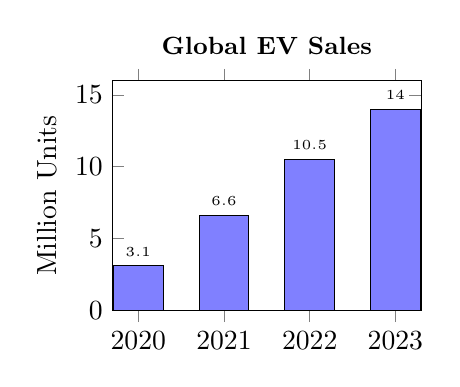
\begin{tikzpicture}
\begin{axis}[
    ybar, bar width=18pt,
    ylabel={Million Units},
    symbolic x coords={2020, 2021, 2022, 2023},
    xtick=data,
    ymin=0, ymax=16,
    width=5.5cm, height=4.5cm,
    nodes near coords,
    every node near coord/.append style={font=\tiny},
    title={\small Global EV Sales},
    title style={font=\small\bfseries}
]
\addplot[fill=blue!50] coordinates {(2020,3.1) (2021,6.6) (2022,10.5) (2023,14.0)};
\end{axis}
\end{tikzpicture}
\end{column}
\end{columns}
\end{frame}

\section{Problem Statement}

\begin{frame}{Current Charging Workflow --- Friction Points}
\begin{columns}
\begin{column}{0.48\textwidth}
\textbf{The 8-Step Manual Process:}
\begin{enumerate}
    \item Arrive at charging station
    \item Identify the charging network
    \item Download operator's app
    \item Create account \& add payment
    \item Scan QR code / enter station ID
    \item Select plan \& confirm
    \item Wait for cloud verification
    \item Charging begins
\end{enumerate}
\end{column}
\begin{column}{0.48\textwidth}
\begin{alertblock}{Vulnerabilities \& Failure Points}
\begin{itemize}
    \item App crashes, forgotten passwords
    \item Poor cellular connectivity (garages)
    \item QR code failures in low light
    \item Multiple operator apps needed
\end{itemize}
\end{alertblock}
\vspace{0.3em}
\begin{exampleblock}{Our Goal}
\textbf{Zero interaction:} Park $\to$ Camera detects plate $\to$ Automatically authorized
\end{exampleblock}
\end{column}
\end{columns}
\end{frame}

\section{Literature Survey}

\begin{frame}{Literature Survey --- Gap Analysis}
\footnotesize
\begin{tabular}{lll}
\toprule
\textbf{Ref. Source} & \textbf{Core Technique} & \textbf{Relevance/Limitation} \\
\midrule
Krishnamoorthi (2018) & CNN Quantization Guide & Guided our INT8 strategy \\
Laroca (2021) & Deep Learning ALPR & Baseline YOLO for plates \\
Zheng (2022) & Edge IoT for EVs & Relies entirely on sensors \\
Lee (2021) & OCPP Smart Scheduling & Lacks automated user auth \\
Hardman (2018) & EV Consumer Preferences & Identified ``app-fatigue'' \\
\bottomrule
\end{tabular}
\vspace{1em}

\begin{block}{The Unsolved Gap}
Existing research focuses either on cloud-based ALPR (which has latency/connectivity issues) or sensor-driven station wellness.
\textbf{No comprehensive local edge-vision solution exists} to bypass the EV authentication bottleneck.
\end{block}
\end{frame}

% ============================================================
% PART 2: ARCHITECTURE (Logical bifurcation 2)
% ============================================================
\section{System Architecture}

\begin{frame}{High-Level System Design}
\centering
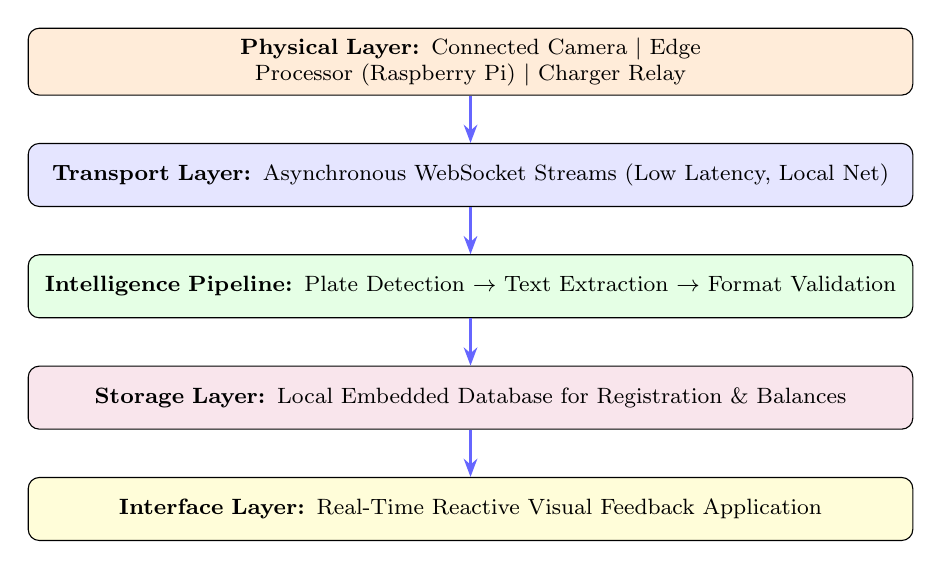
\begin{tikzpicture}[
    node distance=1cm and 2cm,
    layer/.style={rectangle, draw, fill=#1, text width=11cm, text centered, minimum height=0.8cm, font=\footnotesize, rounded corners},
    arrow/.style={thick,->,>=Stealth}
]
    \node [layer=orange!15] (hw) {\textbf{Physical Layer:} Connected Camera $|$ Edge Processor (Raspberry Pi) $|$ Charger Relay};
    \node [layer=blue!10, below=0.6cm of hw] (comm) {\textbf{Transport Layer:} Asynchronous WebSocket Streams (Low Latency, Local Net)};
    \node [layer=green!10, below=0.6cm of comm] (proc) {\textbf{Intelligence Pipeline:} Plate Detection $\to$ Text Extraction $\to$ Format Validation};
    \node [layer=purple!10, below=0.6cm of proc] (data) {\textbf{Storage Layer:} Local Embedded Database for Registration \& Balances};
    \node [layer=yellow!15, below=0.6cm of data] (ui) {\textbf{Interface Layer:} Real-Time Reactive Visual Feedback Application};
    
    \draw [arrow, blue!60] (hw) -- (comm);
    \draw [arrow, blue!60] (comm) -- (proc);
    \draw [arrow, blue!60] (proc) -- (data);
    \draw [arrow, blue!60] (data) -- (ui);
\end{tikzpicture}
\end{frame}

\begin{frame}{End-to-End Data Flow}
\begin{columns}
\begin{column}{0.5\textwidth}
\begin{block}{The Pipeline Process}
\begin{enumerate}
    \item \textbf{Capture:} Camera fetches frame.
    \item \textbf{Transmit:} Raw stream sent to edge node.
    \item \textbf{Identify:} Model draws bounding box.
    \item \textbf{Digitize:} AI reads the text characters.
    \item \textbf{Format Check:} Enforce plate syntax logic.
    \item \textbf{Verify:} Query local registry records.
    \item \textbf{Actuate:} Grant charging \& notify user.
\end{enumerate}
\end{block}
\end{column}
\begin{column}{0.45\textwidth}
\begin{exampleblock}{Design Advantages}
\begin{itemize}
    \item \textbf{Completely App-Free} at station
    \item \textbf{Offline Capable} local network
    \item \textbf{Privacy Secured} plate images remain local
\end{itemize}
\end{exampleblock}
\end{column}
\end{columns}
\end{frame}

\begin{frame}{Application UX Flow}
\centering
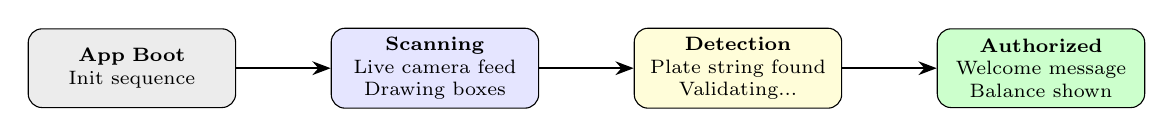
\begin{tikzpicture}[node distance=0.8cm and 1.2cm,
    screen/.style={rectangle, draw, fill=#1, text width=2.4cm, text centered, rounded corners=5pt, minimum height=1cm, font=\scriptsize},
    arrow/.style={thick,->,>=Stealth}]
    
    \node [screen=gray!15] (launch) {\textbf{App Boot}\\Init sequence};
    \node [screen=blue!10, right=of launch] (scan) {\textbf{Scanning}\\Live camera feed\\Drawing boxes};
    \node [screen=yellow!15, right=of scan] (detect) {\textbf{Detection}\\Plate string found\\Validating...};
    \node [screen=green!20, right=of detect] (success) {\textbf{Authorized}\\Welcome message\\Balance shown};
    
    \draw [arrow] (launch) -- (scan);
    \draw [arrow] (scan) -- (detect);
    \draw [arrow] (detect) -- (success);
\end{tikzpicture}

\vspace{1em}
\begin{itemize}
    \item \textbf{Invisible Operation:} The UX flow represents the backend event loop visually. Users don't actually need to open an app at the station.
    \item \textbf{Responsive Feedback:} Visual boundaries turn green upon validation, providing immediate certainty to the station operator or driver.
\end{itemize}
\end{frame}

% ============================================================
% PART 3: DATABASE (Logical bifurcation 3)
% ============================================================
\section{Database Design}

\begin{frame}{Database Structure}
\centering
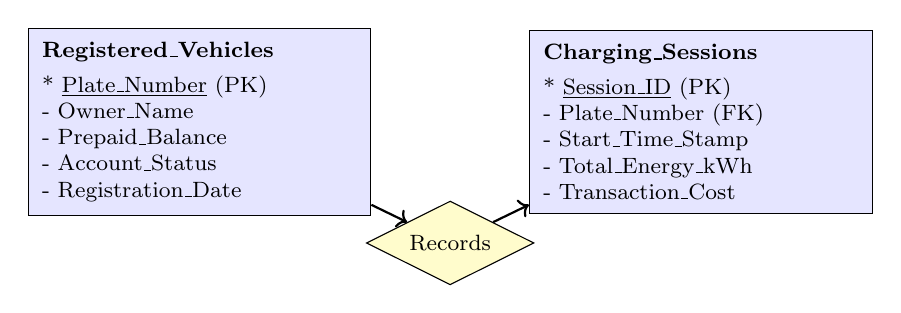
\begin{tikzpicture}[
    entity/.style={rectangle, draw, fill=blue!10, text width=4cm, font=\footnotesize, minimum height=2.2cm, align=left, inner sep=5pt},
    rel/.style={diamond, draw, fill=yellow!20, font=\footnotesize, aspect=2}
]
    \node [entity] (vehicle) {
        \textbf{Registered\_Vehicles}\\[3pt]
        * \underline{Plate\_Number} (PK)\\
        - Owner\_Name\\
        - Prepaid\_Balance\\
        - Account\_Status\\
        - Registration\_Date
    };
    \node [entity, right=2cm of vehicle] (session) {
        \textbf{Charging\_Sessions}\\[3pt]
        * \underline{Session\_ID} (PK)\\
        - Plate\_Number (FK)\\
        - Start\_Time\_Stamp\\
        - Total\_Energy\_kWh\\
        - Transaction\_Cost
    };
    \node [rel, below=1cm of $(vehicle)!0.5!(session)$] (has) {Records};
    \draw [->,thick] (vehicle) -- (has);
    \draw [->,thick] (has) -- (session);
\end{tikzpicture}

\vspace{0.5em}
Implemented via \textbf{SQLite}: Lightweight, Serverless, Zero-Configuration.
\end{frame}

\begin{frame}{Verification \& Integrity Workflow}
\begin{columns}
\begin{column}{0.48\textwidth}
\begin{block}{Verification Rules}
\begin{enumerate}
    \item \textbf{Existence Check:} Does the license plate exist in the registry?
    \item \textbf{Status Check:} Is the account marked `Active'?
    \item \textbf{Financial Check:} Is the prepaid balance $> 0$?
\end{enumerate}
If \textbf{all} tests pass, authorization is triggered and an active session begins.
\end{block}
\end{column}
\begin{column}{0.48\textwidth}
\begin{block}{Security \& Performance}
\begin{itemize}
    \item \textbf{Atomicity:} Cost deduction and session logging behave as a single transaction unit.
    \item \textbf{Constrains:} Foreign key relation prevents ghost sessions.
    \item \textbf{Speed:} Simple primary-key string lookups yield response times under 1 millisecond.
\end{itemize}
\end{block}
\end{column}
\end{columns}
\end{frame}

\begin{frame}{SQLite vs. Cloud-Based Storage}
\begin{columns}
\begin{column}{0.48\textwidth}
\begin{alertblock}{The Cloud Bottleneck}
Connecting to a cloud database (Firebase, AWS RDS) introduces:
\begin{itemize}
    \item 200--500\,ms of network latency per query.
    \item 100\% dependency on 4G/5G cellular connectivity.
    \item Potential data privacy risks from transmitting license plates over public networks.
\end{itemize}
\end{alertblock}
\end{column}
\begin{column}{0.48\textwidth}
\begin{exampleblock}{The Edge Storage Advantage}
By embedding \textbf{SQLite3} directly onto the Raspberry Pi:
\begin{itemize}
    \item \textbf{Latency:} Query execution drops to $< 1$\,ms.
    \item \textbf{Reliability:} The station operates perfectly in subterranean garages with zero signal.
    \item \textbf{Autonomy:} Complete ``Offline-First'' architecture.
\end{itemize}
\end{exampleblock}
\end{column}
\end{columns}
\end{frame}

\begin{frame}{Database Query Execution Loop}
\begin{columns}
\begin{column}{0.48\textwidth}
\textbf{The Evaluation Cycle:}
When Python receives a validated regex plate string, it executes the following logic gate:
\vspace{0.8em}

\begin{enumerate}
    \item \textbf{Lookup:} \texttt{SELECT *} on vehicles.
    \item \textbf{Result Pool:} 
    \begin{itemize}
        \item If \textit{Empty}: Ignore / Log failure.
        \item If \textit{Match}: Proceed to Step 3.
    \end{itemize}
    \item \textbf{Authorize:} Check if \texttt{balance $>$ 0} AND \texttt{status == `active'}.
    \item \textbf{Transact:} Start Charging Session and lock DB row.
\end{enumerate}
\end{column}
\begin{column}{0.48\textwidth}
\centering
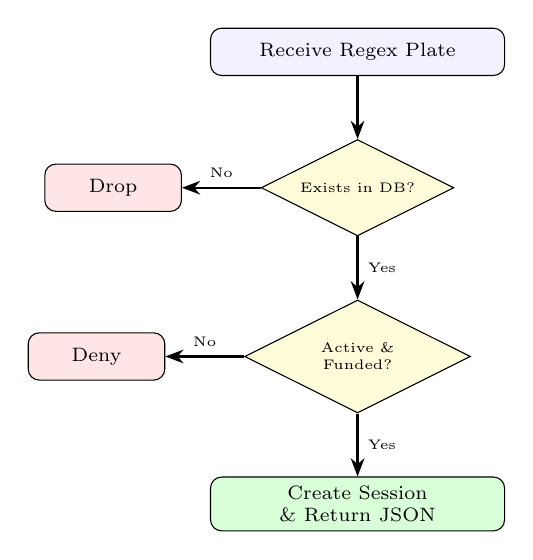
\begin{tikzpicture}[node distance=0.8cm,
    block/.style={rectangle, draw, fill=blue!5, text width=3.5cm, text centered, rounded corners, minimum height=0.6cm, font=\scriptsize},
    decision/.style={diamond, draw, fill=yellow!15, text width=1.5cm, text centered, aspect=2, font=\tiny},
    arrow/.style={thick,->,>=Stealth}]
    
    \node [block] (input) {Receive Regex Plate};
    \node [decision, below=of input] (exist) {Exists in DB?};
    \node [block, left=1cm of exist, fill=red!10, text width=1.5cm] (drop) {Drop};
    \node [decision, below=of exist] (auth) {Active \& Funded?};
    \node [block, left=1cm of auth, fill=red!10, text width=1.5cm] (deny) {Deny};
    \node [block, below=of auth, fill=green!15] (grant) {Create Session\\\& Return JSON};
    
    \draw [arrow] (input) -- (exist);
    \draw [arrow] (exist) -- node[above, font=\tiny]{No} (drop);
    \draw [arrow] (exist) -- node[right, font=\tiny]{Yes} (auth);
    \draw [arrow] (auth) -- node[above, font=\tiny]{No} (deny);
    \draw [arrow] (auth) -- node[right, font=\tiny]{Yes} (grant);
\end{tikzpicture}
\end{column}
\end{columns}
\end{frame}

% ============================================================
% PART 4: QUANTIZATION (Logical bifurcation 4)
% ============================================================
\section{Model Quantization}

\begin{frame}{The Need for Quantization}
\begin{columns}
\begin{column}{0.5\textwidth}
\textbf{The Edge Constraint:}
Running the standard YOLO deep learning model on a Raspberry Pi's CPU brings high latency and exhausts memory limits.

\vspace{0.8em}
\begin{block}{Strategic Approach: INT8}
We converted the model from 32-bit Floating Point (FP32) to 8-bit Integer (INT8).
\begin{itemize}
    \item Compresses file size significantly.
    \item Math uses integer arithmetic instead of fractional calculations.
    \item Utilizes ARM CPU vectorized instructions precisely.
\end{itemize}
\end{block}
\end{column}
\begin{column}{0.45\textwidth}
\centering
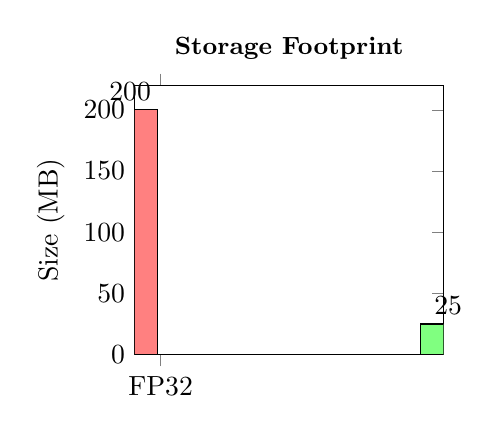
\begin{tikzpicture}
\begin{axis}[
    ybar, bar width=20pt,
    ylabel={Size (MB)},
    symbolic x coords={FP32, INT8},
    xtick=data,
    ymin=0, ymax=220,
    width=5.5cm, height=5cm,
    nodes near coords,
    title={\small Storage Footprint},
    title style={font=\small\bfseries}
]
\addplot[fill=red!50] coordinates {(FP32, 200)};
\addplot[fill=green!50] coordinates {(INT8, 25)};
\end{axis}
\end{tikzpicture}
\end{column}
\end{columns}
\end{frame}

\begin{frame}{Solving the ARM Compatibility Challenge}
\begin{columns}
\begin{column}{0.55\textwidth}
\begin{alertblock}{Hardware Rejection}
ARM CPU instructions explicitly drop support for \textbf{signed} 8-bit convolutions. Standard compiler quantization breaks on the Raspberry Pi.
\end{alertblock}

\vspace{0.3em}

\begin{exampleblock}{Our Graph Patching Tool}
Programmatic intervention without retraining:
\begin{itemize}
    \item Script reads the compiled neural network graph.
    \item Targets all Convolutional nodes.
    \item Mathematically shifts signed arrays $[-128, 127]$ to unsigned domain $[0, 255]$.
    \item Overwrites zero-point tensors and saves.
\end{itemize}
\end{exampleblock}
\end{column}
\begin{column}{0.4\textwidth}
\centering
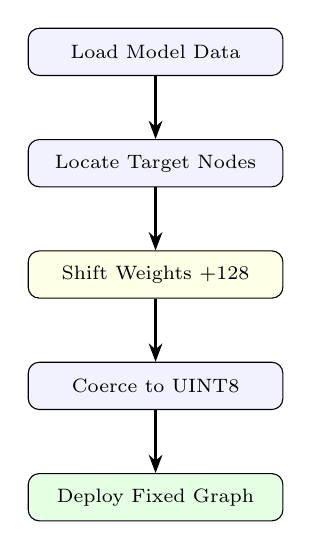
\begin{tikzpicture}[node distance=0.8cm,
    block/.style={rectangle, draw, fill=blue!5, text width=3cm, text centered, rounded corners, minimum height=0.6cm, font=\scriptsize},
    arrow/.style={thick,->,>=Stealth}]
    \node [block] (load) {Load Model Data};
    \node [block, below=of load] (find) {Locate Target Nodes};
    \node [block, below=of find, fill=yellow!10] (shift) {Shift Weights +128};
    \node [block, below=of shift] (replace) {Coerce to UINT8};
    \node [block, below=of replace, fill=green!10] (save) {Deploy Fixed Graph};
    \draw [arrow] (load) -- (find);
    \draw [arrow] (find) -- (shift);
    \draw [arrow] (shift) -- (replace);
    \draw [arrow] (replace) -- (save);
\end{tikzpicture}
\end{column}
\end{columns}
\end{frame}

\begin{frame}{OCR Text Extraction Pipeline}
\begin{columns}
\begin{column}{0.5\textwidth}
\textbf{From Pixels to Text:}
Once YOLO detects the license plate, the coordinate bounding box is used to crop the image. This crop is passed to the OCR subsystem.

\vspace{0.8em}
\begin{block}{EasyOCR Engine}
\begin{itemize}
    \item \textbf{Text Detection:} CRAFT (Character Region Awareness for Text).
    \item \textbf{Text Recognition:} CRNN (Convolutional Recurrent Neural Network).
    \item \textbf{Benefits:} Lightweight, highly accurate on alphanumeric characters without heavy GPU dependence.
\end{itemize}
\end{block}
\end{column}
\begin{column}{0.45\textwidth}
\centering
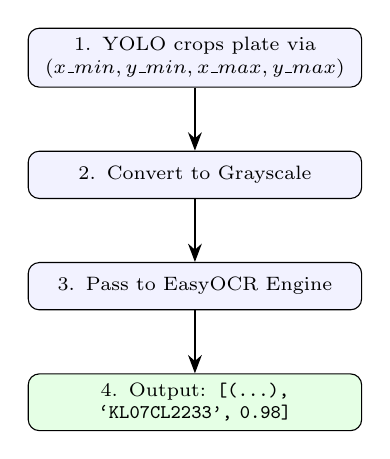
\begin{tikzpicture}[node distance=0.8cm,
    block/.style={rectangle, draw, fill=blue!5, text width=4cm, text centered, rounded corners, minimum height=0.6cm, font=\scriptsize},
    arrow/.style={thick,->,>=Stealth}]
    \node [block] (crop) {1. YOLO crops plate via $(x\_min, y\_min, x\_max, y\_max)$};
    \node [block, below=of crop] (grey) {2. Convert to Grayscale};
    \node [block, below=of grey] (easy) {3. Pass to EasyOCR Engine};
    \node [block, below=of easy, fill=green!10] (result) {4. Output: \texttt{[(\dots), `KL07CL2233', 0.98]}};
    \draw [arrow] (crop) -- (grey);
    \draw [arrow] (grey) -- (easy);
    \draw [arrow] (easy) -- (result);
\end{tikzpicture}
\end{column}
\end{columns}
\end{frame}

\begin{frame}{Regex Filtering and Formatting}
\begin{block}{The Noise Problem}
OCR systems often pick up stray characters from license plate frames, screws, or state emblems. We must filter this noise before database verification.
\end{block}

\begin{columns}
\begin{column}{0.48\textwidth}
\begin{exampleblock}{Validation Strategy}
\begin{enumerate}
    \item \textbf{Sanitize:} Remove all spaces and non-alphanumeric characters.
    \item \textbf{Regex Match:} Apply strict formatting rules for Indian license plates.
    \item \textbf{Reject/Accept:} Only perfectly matched patterns proceed to the database.
\end{enumerate}
\end{exampleblock}
\end{column}
\begin{column}{0.48\textwidth}
\centering
\textbf{Indian Format Regex:}\\
\vspace{0.5em}
\texttt{\^{}[A-Z]\{2\}[0-9]\{2\}[A-Z]\{1,2\}[0-9]\{4\}\$}

\vspace{0.8em}
\begin{tabular}{ll}
\toprule
\textbf{Raw OCR Output} & \textbf{Final Result} \\
\midrule
``KL 07 CL 2233'' & \texttt{KL07CL2233} \\
``IND KL07 CL2233.'' & \texttt{KL07CL2233} \\
``K1O7CL2233'' & \textcolor{red}{\textsl{Rejected}} \\
\bottomrule
\end{tabular}
\end{column}
\end{columns}
\end{frame}

% ============================================================
% PART 5: IMPLEMENTATION & PACKAGES (Logical bifurcation 1 returned)
% ============================================================
\section{Implementation \& Packages}

\begin{frame}{Key Libraries and Frameworks Used}
\begin{columns}
\begin{column}{0.48\textwidth}
\begin{block}{Python Ecosystem (Edge Node)}
\begin{itemize}
    \item \textbf{asyncio \& websockets:} For non-blocking, multi-client, full-duplex TCP routing.
    \item \textbf{OpenCV (cv2) \& numpy:} Matrix array processing, frame decoding, and bounds drawing.
    \item \textbf{onnxruntime:} Highly optimized C++ backend engine for executing ARM INT8 inferences.
    \item \textbf{EasyOCR:} Character extraction engine built atop PyTorch principles.
    \item \textbf{re \& sqlite3:} Regex text sanitization and local database execution.
\end{itemize}
\end{block}
\end{column}
\begin{column}{0.48\textwidth}
\begin{block}{Swift Ecosystem (iOS Client Node)}
\begin{itemize}
    \item \textbf{SwiftUI \& Combine:} Reactive native component framework using `@Published` wrappers.
    \item \textbf{AVFoundation:} Hardware-level interaction to capture and delegate live camera buffer streams.
    \item \textbf{CoreImage:} Immediate conversion of binary feed blocks into compressed structural JPEG payloads.
    \item \textbf{Foundation (JSONDecoder):} Secure polymorphic conversion from text blocks back into strict memory structs.
\end{itemize}
\end{block}
\end{column}
\end{columns}
\end{frame}

\begin{frame}{Crucial Project Functions}
\footnotesize
\begin{table}[H]
\centering
\renewcommand{\arraystretch}{1.2}
\begin{tabular}{p{3.5cm} p{1.8cm} p{8.5cm}}
\toprule
\textbf{Function Name} & \textbf{Domain} & \textbf{Purpose} \\
\midrule
\texttt{decode\_image()} & Python & Converts binary payload to BGR matrix asynchronously \\
\texttt{handle\_connection()} & Python & Coroutine managing crop, OCR, and WS transmission \\
\texttt{fix\_conv\_integer()} & Python & ONNX script that corrects signed INT8 incompatibilities \\
\texttt{validate\_plate()} & Python & Detaches spaces and runs regex on Indian plate layouts \\
\texttt{captureOutput()} & Swift & Delegate intercepting raw pixel buffers from device lens \\
\texttt{handleResponse()} & Swift & Decoder gracefully dropping frame info upon auth success \\
\bottomrule
\end{tabular}
\end{table}
\end{frame}

% ============================================================
% RESULTS
% ============================================================
\section{Results}

\begin{frame}{Latency \& Execution Benchmarks}
\begin{columns}
\begin{column}{0.48\textwidth}
\begin{block}{CPU Execution Yield}
\begin{itemize}
    \item FP32 Base Inference: \textbf{1842 ms.}
    \item Custom INT8 Inference: \textbf{487 ms.}
    \item \textbf{3.78$\times$ Speed Increase}.
    \item Real impact: Achieves capable 2$+$ FPS directly on micro-SBC.
\end{itemize}
\end{block}
\begin{block}{Memory Constrictions}
\begin{itemize}
    \item FP32 RAM Overhead: $\approx 1.28$ GB
    \item INT8 RAM Overhead: $\approx 478$ MB
    \item Fits entirely inside constraints with zero OS-level page swaps.
\end{itemize}
\end{block}
\end{column}
\begin{column}{0.48\textwidth}
\centering
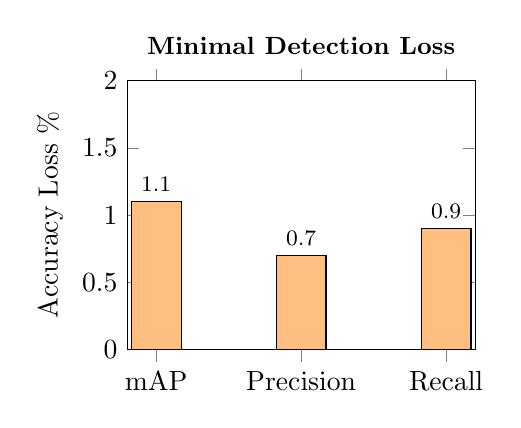
\begin{tikzpicture}
\begin{axis}[
    ybar, bar width=18pt,
    ylabel={Accuracy Loss \%},
    symbolic x coords={mAP, Precision, Recall},
    xtick=data,
    ymin=0, ymax=2,
    width=6cm, height=5cm,
    nodes near coords,
    every node near coord/.append style={font=\footnotesize},
    title={\small Minimal Detection Loss},
    title style={font=\small\bfseries}
]
\addplot[fill=orange!50] coordinates {(mAP, 1.1) (Precision, 0.7) (Recall, 0.9)};
\end{axis}
\end{tikzpicture}

\textit{Virtually indistinguishable precision compared to the huge baseline model.}
\end{column}
\end{columns}
\end{frame}

\section{Conclusion}

\begin{frame}{Conclusion \& Future Scope}
\begin{block}{System Advantages Validated}
\begin{itemize}
    \item Successfully eliminated the 8-step app process down to \textbf{zero steps}.
    \item Eliminated cloud dependence; works 100\% offline.
    \item Overcame IoT hardware limitations through direct mathematical model manipulation.
\end{itemize}
\end{block}

\begin{block}{Future Trajectory}
\begin{itemize}
    \item \textbf{Relay Actioning:} Connect the edge Pi's physical GPIO pins to the charger relays.
    \item \textbf{Interoperability:} Hook the local DB into OCPP 2.0.1 for global billing sync while maintaining local auth speeds.
    \item \textbf{Broader Detection:} Include US/EU format regex parameters and expand PaddleOCR parsing capabilities.
\end{itemize}
\end{block}
\end{frame}

\begin{frame}
\centering
\vspace{1.5cm}
{\Huge \textbf{Thank You!}}

\vspace{1cm}
{\large Questions?}

\vspace{1.5cm}
\begin{tabular}{c c c c}
\textbf{Joel K George} & \textbf{Sarah Ann Pothen} & \textbf{Shahma Fathima} & \textbf{Izz al Din Noufel}
\end{tabular}

\vspace{0.8em}
{\footnotesize Project Guide: \textbf{Dr. Manju K}}
\end{frame}

\end{document}
